\section{Пример: лютеинизирующий гормон}

На рис. 8.4 показан набор данных про уровень $y_t$ лютенизирующего гормона для каждого из $48$ отрезков времени, взятых из Diggle (1990); набор данных приведен в таблице 8.1. Это данные об уровне гормона, измеренные у здоровой женщины с $10$-минутными интервалами в течение $8$ часов. Лютенизирующий гормон является одним из гормонов, регулирующих менструальный цикл, и поэтому важно понимать его суточные колебания. 

Понятно, что уровни гормона не являются случайной выборкой из какого-либо распределения. На рисунке 8.4 слишком много данных. Эти данные являются примером \textit{временного ряда}: структуры данных, для которой близкие значения временного параметра $t$ указывают тесно связанные значения измеренной величины $y_t$. Для анализа временных рядов используются многие интересные вероятностные модели. Мы начнем с простейшей модели~--- \textit{схемы авторегрессии первого порядка}.

Пусть $\mu$ --- математическое ожидание $y_t$, которое предполагается одинаковым для всех моментов времени $t$, и определим \textit{центрированные} измерения
\begin{equation}
	z_t = y_t - \mu.
\end{equation}
Все $z_t$ имеют математическое ожидание $0$. Схема авторегрессии первого порядка --- это одна из таких схем, в которой каждый $z_t$ является линейной комбинацией предыдущего значения $z_{t-1}$ и независимого шума $\varepsilon_t$,
\begin{equation}
	z_t = \beta z_{t-1} + \varepsilon_t \text{ для } t = U, U + 1, U + 2, \ldots, V.
\end{equation}
\\[0.5cm]
\noindent
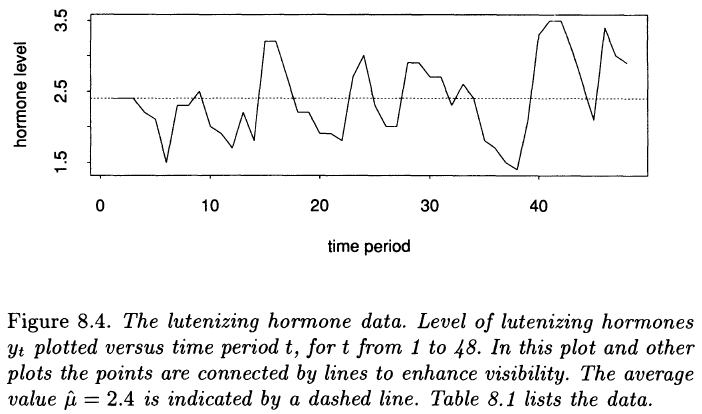
\includegraphics[width=12cm]{8/f84}
\newline
\noindent Здесь $\beta$ --- неизвестный параметр, действительное число от $-1$ до $1$. 

Предполагается, что шум $\varepsilon_t$ в (8.15) является случайной выборкой из неизвестного распределения $F$ с математическим ожиданием $0$,
\begin{equation}
	F \to (\varepsilon_U, \varepsilon_{U+1}, \varepsilon_{U+2}, \ldots, \varepsilon_V) \quad [\text{E}_F(\varepsilon) = 0].
\end{equation}
Точки $U$ и $V$ --- это начало и конец анализируемого периода времени. Здесь у нас есть
\begin{equation}
	U = 2 \quad \text{и} \quad V = 48.
\end{equation}
Обратите внимание, что первое уравнение в (8.15) имеет вид
\begin{equation}
	z_U = \beta z_{U-1} + \varepsilon_U,
\end{equation}
поэтому нам нужно число $z_{U-1}$, чтобы запустить процесс авторегрессии. В нашем случае $z_{U-1} = z_1$. 

Пусть мы считаем, что модель (8.15), (8.16), авторегрессионный процесс первого порядка, применима к данным лютенизирующего гормона. Как мы можем оценить значение $\beta$ по данным? Один из ответов основан на методе наименьших квадратов. Прежде всего, мы оцениваем математическое ожидание $\mu$ в (8.14) по наблюдаемому среднему значению $\bar{y}$ (это $2.4$ для данных лютенизирующего гормона) и задаем
\begin{equation}
	z_t = y_t - \bar{y}
\end{equation}
для всех значений $t$. В дальнейшем мы проигнорируем разницу между определениями (8.14) и (8.19). 

Предположим, что $b$ --- это любое предположение об истинном значении $\beta$ в (8.15). Определим остаточную квадратичную ошибку для этого предположения как
\begin{equation}
	\text{RSE}(b) = \sum_{t=U}^{V} (z_t - b_{z_{t-1}})^2.
\end{equation}
Используя (8.15) и тот факт, что $\text{E}_F(\varepsilon) = 0$, легко показать, что $\text{RSE}(b)$ имеет математическое ожидание 
\begin{equation*}
	\text{E}\left(\text{RSE}(b)\right) = (b-\beta)^2 \text{E} \left(\sum_{t=U}^{V} z_{t-1}^2 \right) + (V-U+1) \text{var}_F(\varepsilon).
\end{equation*}
 Оно минимизируется, когда $b$ равно истинному значению $\beta$. Мы убедились, что $\text{RSE}(b)$ должен достичь своего минимума где-то рядом с истинным значением $\beta$. 

Учитывая данные временного ряда, мы можем рассчитать $\text{RSE}(b)$ как функцию $b$, и выбрать минимизирующее значение, которое будет нашей оценкой $\beta$
\begin{equation}
	\text{RSE}(\hat{\beta}) = \min_b \text{RSE}(b).
\end{equation}
Данные про лютенизирующий гормон имеют следующую оценку наименьших квадратов
\begin{equation}
	\hat{\beta} = 0.586.
\end{equation}

Насколько точна оценка $\hat{\beta}$? Чтобы ответить на этот вопрос, мы можем использовать общую бутстреп процедуру, показанную на рис. 8.3. Вероятностный механизм $P$, описанный в (8.15), (8.16), имеет два неизвестных элемента, $\beta$ и $F$, скажем, $P = (\beta, F)$. (Здесь мы рассматриваем $\mu$ в (8.14) как известную и равную $\bar{y}$.) Данные $\textbf{x}$ состоят из наблюдений $y_t$ и соответствующих им периодов времени $t$. Мы знаем, что правило построения $P \to \textbf{x}$ описывается формулами (8.15)--(8.16). Интересующая статистика $\hat{\theta}$ равна $\hat{\beta}$, поэтому отображения $s(\cdot)$ неявно задаются (8.21).

Остается один шаг, прежде чем мы сможем применить бутстреп: шаг двойной стрелки $\textbf{x} \Rightarrow \hat{P}$, в котором $P = (\beta, F)$ оценивается по данным. Теперь $\beta$ уже была оценена с помощью $\hat{\beta}$, (8.21), поэтому нам нужно только оценить распределение отклонений $F$. Если бы мы знали $\beta$, то мы могли бы вычислить $\varepsilon_t = z_t - \beta z_{t-1}$ для каждого $t$ и оценить $F$ по эмпирическому распределению значений $\varepsilon_t$. Мы не знаем $\beta$, то мы можем использовать оценочное значение $\hat{\beta}$, чтобы вычислить \textit{отклонения [approximate disturbances]}
\begin{equation}
	\hat{\varepsilon}_t = z_t - \hat{\beta} z_{t-1} \text{ для } t = U, U + 1, U + 2, \ldots, V.
\end{equation}
Пусть $T = V - U + 1$, количество слагаемых в (8.23); $T = 47$ для выбора (8.17). Очевидная оценка $F$ --- это $\hat{F}$, эмпирическое распределение отклонений
\begin{equation}
	\hat{F}: \text{ вероятность } 1/T \text{ для } \hat{\varepsilon}_t \text{ при } t = U, U + 1, \ldots, V.
\end{equation}

На рис. 8.5 показана гистограмма отклонений $\hat{\varepsilon}_t = z_t - \hat{\beta} z_{t-1}$ с $T = 47$ для схемы авторегрессии первого порядка, примененной к данным о лютеинизирующем гормоне в промежутке от 2 до 48 лет.

\noindent
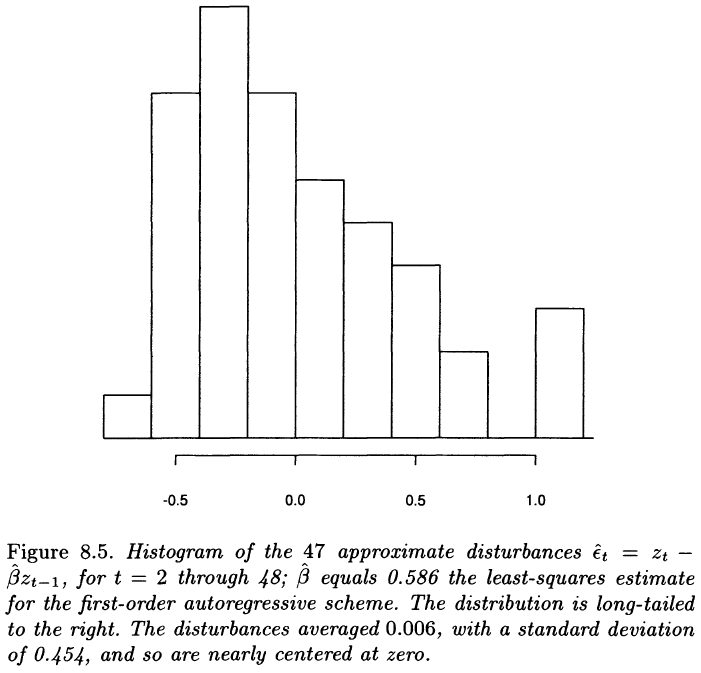
\includegraphics[width=\linewidth]{8/f85}
\newline

Мы видим, что распределение $\hat{F}$ не является нормальным и имеет длинный хвост справа. Распределение имеет среднее значение $0.006$ и стандартное отклонение $0.454$. Не случайно, что среднее значение $\hat{F}$ близко к $0$. Если бы это было не так, мы могли бы соблюдать определение $\text{E}_F(\varepsilon) = 0$ в (8.16) путём центрирования $\hat{F}$; то есть изменением каждой вероятностной точки в (8.23) от $\hat{\varepsilon}_t$ до $\hat{\varepsilon}_t - \bar{\varepsilon}$, где $\bar{\varepsilon} = \sum_{t=U}^{V} \hat{\varepsilon}_t/T$.

Теперь мы готовы провести бутстреп анализ точности оценки $\hat{\beta} = 0.586$. Набор бутстреп данных $\hat{P} \to \textbf{x}^*$ генерируется в соответствии с определениями (8.15)--(8.16), за исключением $\hat{P} = (\hat{\beta}, \hat{F})$, заменённого на $P = (\beta, F)$. Начнем с начального значение $z_1 = y_1 - \bar{y}$, которое считается фиксированной константой (как размер выборки $n$ в одновыборочной задаче). Бутстреп временной ряд $z_t^*$ вычисляется рекурсивно
\begin{align}
	z_2^* & = \hat{\beta} z_1 + \varepsilon_2^* \notag \\
	z_3^* & = \hat{\beta} z_2^* + \varepsilon_3^* \notag \\
	z_4^* & = \hat{\beta} z_3^* + \varepsilon_4^* \notag \\
	\vdots & \notag \\
	z_{48}^* & = \hat{\beta} z_{47}^* + \varepsilon_{48}^*.
\end{align}
Бутстреп остатки $\varepsilon_t^*$ представляют собой случайную выборку из $\hat{F}$,
\begin{equation}
	\hat{F} \to (\varepsilon_2^*, \varepsilon_2^*, \ldots, \varepsilon_{48}^*).
\end{equation}
Другими словами, каждый $\varepsilon_t^*$ равняется любому из $T$ отклонений (8.23) с вероятностью $1/T$.

Процесс бутстрепа (8.25)--(8.26) был запущен $B=200$ раз, что дало $200$ бутстреп временных рядов. Каждый из них дал бутстреп репликацию $\hat{\beta}^*$ для оценки $\hat{\beta}$ методом наименьших квадратов, (8.21). На рисунке 8.6 показана гистограмма из $200$ значений $\hat{\beta}^*$. Оценка бутстреп стандартной ошибки для $\hat{\beta}$ составляет $\hat{\text{se}}_{200} = 0.116$. Гистограмма имеет довольно нормальную форму.

В схеме авторегрессии первого порядка каждый $z_t$ зависит от своих предшественников только через значение $z_{t-1}$ (Этот вид зависимости известен как \textit{марковский процесс первого порядка}.) Схема авторегрессии второго порядка расширяет зависимость обратно до $z_{t-2}$,
\begin{align}
	z_t = \beta_1 z_{t-1} + \beta_2 z_{t-2} + \varepsilon_t \notag \\
	\text{для } t = U, U + 1, U + 2, \ldots, V.
\end{align}
Здесь $\bm \beta = (\beta_1, \beta_2)^\text{T}$ --- двумерный вектор неизвестных параметров. $\varepsilon_t$ --- независимые отклонения, как в (8.16). Согласно (8.18) исходные уравнения следующие 
\begin{align}
	z_U & = \beta_1 z_{U-1} + \beta_2 z_{U-2} + \varepsilon_U \notag \\
	z_{U+1} & = \beta_1 z_U + \beta_2 z_{U-1} + \varepsilon_{U+1},
\end{align}
поэтому нам нужны числа $z_{U-2}$ и $z_{U-1}$ для начала. Теперь $U = 3$, $V = 48$ и $T = V - U + 1 = 46$.

Метод наименьших квадратов непосредственно приводит к оценке вектора $\bm{\beta}$. Пусть $\textbf{z}$ является $T$-мерным вектором $(z_U, z_{U+1}, \ldots, z_V)^\text{T}$, и пусть $\textbf{Z}$~--- матрица $T \times 2$ с первым столбцом $(z_{U-1}, z_U, \ldots, z_{V-1})^\text{T}$, вторым столбцом $(z_{U-2}, z_{U-1}, z_U,  \ldots, z_{V-2})^\text{T}$. Тогда оценка $\bm{\beta}$ методом наименьших квадратов следующая
\begin{equation}
	\hat{\bm \beta} = (\textbf{Z}^\text{T} \textbf{Z})^{-1} \textbf{Z}^\text{T} \textbf{z}.
\end{equation}

\noindent
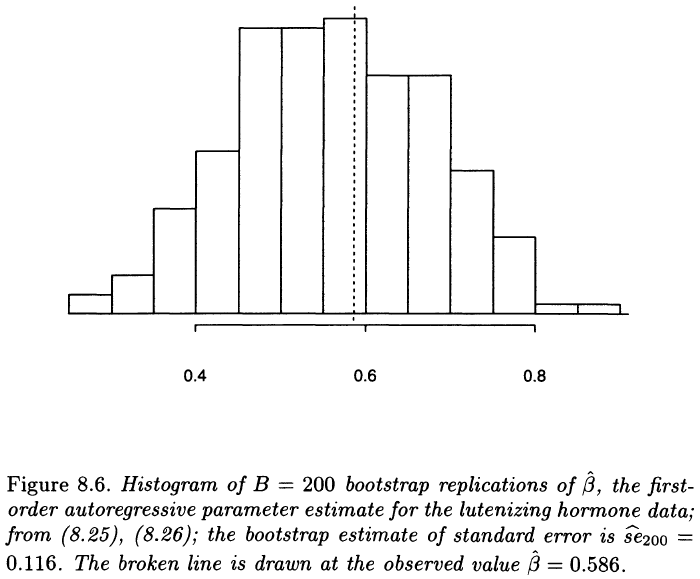
\includegraphics[width=\linewidth]{8/f86}
\newline

Для данных о лютенизирующем гормоне схема авторегрессии второго порядка имела следующие оценки наименьших квадратов
\begin{equation}
	\hat{\bm \beta} = (0.771, -0.222)^\text{T}.
\end{equation}
На рис. 8.7 показаны гистограммы с $B=200$ бутстреп репликациями из двух компонентов из $\hat{\bm \beta} = (\hat{\beta}_1, \hat{\beta}_2)^\text{T}$. Стандартные ошибки бутстрепа равны
\begin{equation}
	\widehat{\text{se}}_{200} (\hat \beta_1) = 0.147, \quad \widehat{\text{se}}_{200} (\hat \beta_2) = 0.149.
\end{equation}
Обе гистограммы приближенно имеют форму нормального распределения.

Схема авторегрессии второго порядка при $\beta_2 = 0$ является схемой авторегрессии первого порядка. При выполнении анализа точности для схемы второго порядка мы проверяем, не отклоняется ли $\hat \beta_2$ от $0$ менее чем на $2$ стандартные ошибки, что обычно интерпретируется как незначительное отличие $\hat \beta_2$ от $0$. Здесь $\hat \beta_2$ --- это примерное отклонение на $1.5$ стандартные ошибки от $0$, и в этом случае у нас нет убедительных доказательств того, что схема авторегрессии первого порядка не дает разумного представления данных о лютеинизирующем гормоне.

Знаем ли мы наверняка, что схема первого порядка дает хорошее представление о ряде лютенизирующих гормонов? Мы не можем дать окончательный ответ на этот вопрос, не рассматривая еще более общие модели,
\\[0.5cm]
\noindent
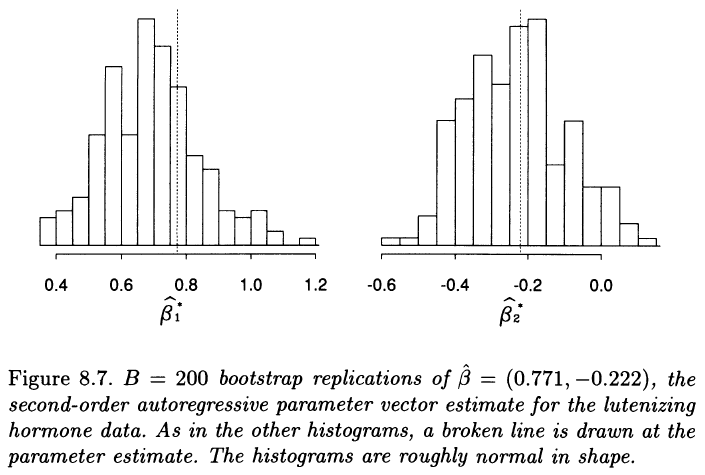
\includegraphics[width=\linewidth]{8/f87}
\newline
такие как схемы авторегрессии более высоких порядков. Приблизительный ответ может быть получен путем сравнения бустреп временных рядов с фактическими рядами на рис. 8.4. На рисунке 8.8 на левых графиках показаны первые четыре бустреп набора из первой схемы, правые четыре графика отображают реализации, полученные путем выборки с повторением из исходного временного ряда. Исходные данные на рис. 8.4 очень похожи на реализации левых графиков и совсем не похожи на реализации правых графиков.

Дальнейший анализ показывает, что модель AR(1) обеспечивает разумное соответствие этим данным. Однако нам потребуется более длительный временной ряд, чтобы эффективно различать разные модели для этого гормона.

В общем, стоит помнить, что математические модели представляют собой удобные упрощенные представления сложных явлений реального мира и иногда не совсем корректны. Часто необходим некоторый компромисс между усложнением модели и научными потребностями исследования. Методы бустрепа особенно полезны, если существует потребность в сложных моделях, поскольку математическая сложность не является препятствием для анализа точности бустрепа.\\